\documentclass{article}
\usepackage[english,russian]{babel}
\usepackage{textcomp}
\usepackage{geometry}
  \geometry{left=2cm}
  \geometry{right=1.5cm}
  \geometry{top=1.5cm}
  \geometry{bottom=2cm}
\usepackage{tikz}
\usepackage{multicol}
\usepackage{listings}
\pagenumbering{gobble}

\lstdefinestyle{csMiptCppStyle}{
  language=C++,
  basicstyle=\linespread{1.1}\ttfamily,
  columns=fixed,
  fontadjust=true,
  basewidth=0.5em,
  keywordstyle=\color{blue}\bfseries,
  commentstyle=\color{gray},
  texcl=true,
  stringstyle=\ttfamily\color{orange!50!black},
  showstringspaces=false,
  numbersep=5pt,
  numberstyle=\tiny\color{black},
  numberfirstline=true,
  stepnumber=1,      
  numbersep=10pt,
  backgroundcolor=\color{white},
  showstringspaces=false,
  captionpos=b,
  breaklines=true
  breakatwhitespace=true,
  xleftmargin=.2in,
  extendedchars=\true,
  keepspaces = true,
  tabsize=4,
  upquote=true,
  emph={override, nullptr},
  emphstyle={\color{blue}},
}


\lstdefinestyle{csMiptCppLinesStyle}{
  style=csMiptCppStyle,
  frame=lines,
}

\lstdefinestyle{csMiptCppBorderStyle}{
  style=csMiptCppStyle,
  framexleftmargin=5mm, 
  frame=shadowbox, 
  rulesepcolor=\color{gray}
}

\lstset{style=csMiptCppStyle}
\lstset{literate={~}{{\raisebox{0.5ex}{\texttildelow}}}{1}}


\renewcommand{\thesection}{\arabic{section}}
\makeatletter
\def\@seccntformat#1{\@ifundefined{#1@cntformat}%
   {\csname the#1\endcsname\quad}%    default
   {\csname #1@cntformat\endcsname}}% enable individual control
\newcommand\section@cntformat{Часть \thesection:\space}
\makeatother


\begin{document}
\title{Семинар \#3: Динамический полиморфизм \vspace{-5ex}}\date{}\maketitle

\section{Полиморфизм}

\begin{description}
\item[Полиморфизм] -- это способность функций обрабатывать данные разных типов.
\end{description}

\noindent Полиморфизм существует в большинстве языков программирования в том или ином виде. Например, рассмотрим следующую программу на языке Python:
\begin{lstlisting}[language=Python]
def plus(a, b):
    return (a + b)
print(plus(10, 20))        # Напечатает 30
print(plus("Cat", "Dog"))  # Напечатает CatDog
\end{lstlisting}
Здесь функция \texttt{plus} является полиморфной, так как может работать с данными разных типов.

\subsection*{Статический полиморфизм}
Полиморфизм в языке C++ мы уже частично прошли. Ведь такие возможности языка как перегрузка функций и шаблоны позволяют писать функции, которые работают с разными типами:
\begin{lstlisting}[style=csMiptCppStyle]
#include <iostream>
#include <string>
using namespace std::string_literals;

template<typename T>
T plus(T x, T y)
{
	return x + y;
}

int main()
{
	std::cout << plus(10, 20) << std::endl;          // Напечатает 30
	std::cout << plus("Cat"s, "Dog"s) << std::endl;  // Напечатает CatDog
}
\end{lstlisting}
Однако, в этом случае, то, какая функция будет вызвана, определяется на этапе компиляции: при раскрытии шаблона или при выборе перегрузки. Вид полиморфизма, при котором вызываемая функция определяется на этапе компиляции, называется статическим полиморфизмом. 
\subsection*{Динамический полиморфизм}
При динамическом полиморфизме то, какая функция будет вызвана определяется на этапе выполнения. Так как мы хотим, чтобы для разных типов вызывались разные функции, то при динамическом полиморфизме на этапе компиляции даже не будет известен тип объекта, приходящего на вход функции, он станет известен только на этапе выполнения. Таким образом в языке должны существовать объекты, которые могут "менять"{} свой тип.\\
В языке Python динамический полиморфизм просто встроен в язык и любые объекты могут менять свой тип:
\begin{lstlisting}[language=Python]
a, b = 10, 20
print(plus(a, b))     # Напечатает 30, тип объектов a и b - int
a, b = "Cat", "Dog"
print(plus(a, b))     # Напечатает CatDog, тип объектов a и b - строка
\end{lstlisting}
В языке С++ у всех объектов фиксированный тип, а динамический полиморфизм достигается с помощью механизмов наследования и виртуальных функций.

\newpage
\section{Виртуальные функции}
Виртуальные функции (также известные как виртуальные методы) -- это механизм, который позволяет осуществлять динамический полиморфизм в языке C++.
Виртуальные функции позволяют динамически определять, какая функция будет вызвана в зависимости от типа объекта, а не типа указателя или ссылки, указывающего на этот объект.
Виртуальные функции не следует путать с виртуальным наследованием, это разные вещи.

Чтобы указать, что метод является виртуальным, нужно использовать ключевое слово \texttt{virtual} в объявлении метода в базовом классе. После этого данный метод, а также все \textit{переопределённые методы} (то есть методы с такими же сигнатурами) во всех производных классах станут виртуальными. Использовать \texttt{virtual} в объявлениях методов производных классов необязательно. Виртуальный метод отличается от обычного следующим:

\begin{center}
\textit{Если в программе возникнет ситуация когда указатель (или ссылка) на базовый класс будет указывать на объект производного класса, то при вызове виртуального метода через этот указатель (или ссылку) будет вызываться метод производного класса, а не метод базового класса.}
\end{center}

Рассмотрим пример класса \texttt{Bob}, который наследуется от класса \texttt{Alice} и у этих классов есть виртуальные методы под названием \texttt{say}. Метод \texttt{say} в классе \texttt{Alice} стал виртуальным, так как мы пометили его ключевым словом \texttt{virtual}. Метод \texttt{say} в классе \texttt{Bob} также будет виртуальным, потому что он переопределяет виртуальный метод в родительском классе. Таким образом, независимо от того пометим мы метод \texttt{Bob::say} словом \texttt{virtual} или нет, он будет виртуальным.


\begin{lstlisting}[style=csMiptCppBorderStyle]
struct Alice 
{
    virtual void say() 
    {
    	std::cout << "Alice" << std::endl;
    }
};

struct Bob : public Alice 
{
    void say() 
    {
    	std::cout << "Bob" << std::endl;
    }
};
\end{lstlisting}
Виртуальные методы отличаются от обычных методов тем, что если мы вызываем этот метод через указатель (или ссылку) на объект, то будет вызываться метод класса объекта на который указывает этот указатель.
\begin{lstlisting}[style=csMiptCppBorderStyle]
Bob b;

Alice* pa = &b;
pa->say();  // Вызовется метод Bob::say, так как pa указывает на объект типа Bob
            // Если бы метод say не был бы виртуальным, то вызвался бы метод Alice::say,
            // так как указатель имеет тип Alice*
            
Alice& ra = b;
ra.say();   // Вызовется метод Bob::say, так как ra указывает на объект типа Bob
            // Если бы метод say не был бы виртуальным, то вызвался бы метод Alice::say,
            
Alice a = b;
a.say();    // Вызовется метод Alice::say (тут виртуальность не работает)
\end{lstlisting}



\noindent Обратите внимание, что виртуальные функции работают в случае когда есть указатель (или ссылка) на базовый класс, который указывает на объект производного класса, но не работают когда, например, объект базового класса инициализирован объектом производного класса.

\newpage
\subsection*{Объект базового класса, инициализированный объектом производного}
\begin{multicols}{2} \noindent
\begin{lstlisting}[style=csMiptCppBorderStyle]
#include <iostream>
struct Alice 
{
    void say() 
    {
    	std::cout << "Alice" << std::endl;
    }
};
struct Bob : public Alice 
{
    void say() 
    {
    	std::cout << "Bob" << std::endl;
    }
};

int main() 
{
    Bob b;
	Alice a = b;
    a.say();  // Напечатает Alice
}
\end{lstlisting}


\begin{lstlisting}[style=csMiptCppBorderStyle]
#include <iostream>
struct Alice 
{
    virtual void say() 
    {
    	std::cout << "Alice" << std::endl;
    }
};
struct Bob : public Alice 
{
    void say() 
    {
    	std::cout << "Bob" << std::endl;
    }
};

int main() 
{
    Bob b;
	Alice a = b;
    a.say();  // Всё равно напечатает Alice
}
\end{lstlisting}
\end{multicols}

\subsection*{Указатели на базовый класс, хранящие адрес объекта производного класса}
\begin{multicols}{2}\noindent
\begin{lstlisting}[style=csMiptCppBorderStyle]
#include <iostream>
struct Alice 
{
    void say() 
    {
    	std::cout << "Alice" << std::endl;
    }
};
struct Bob : public Alice 
{
    void say() 
    {
    	std::cout << "Bob" << std::endl;
    }
};

int main() 
{
    Bob b;
	Alice* pa = &b;
    pa->say();  // Напечатает Alice
}
\end{lstlisting}


\begin{lstlisting}[style=csMiptCppBorderStyle]
#include <iostream>
struct Alice 
{
    virtual void say() 
    {
    	std::cout << "Alice" << std::endl;
    }
};
struct Bob : public Alice 
{
    void say() 
    {
    	std::cout << "Bob" << std::endl;
    }
};

int main() 
{
    Bob b;
	Alice* pa = &b;
    pa->say();  // Напечатает Bob
}
\end{lstlisting}
\end{multicols}

\newpage
\subsection*{Как виртуальные функции приводят к динамическому полиморфизму}
Указатель типа \texttt{Alice*} может указывать как на объект типа \texttt{Alice} или на объект типа \texttt{Bob} (или на объект любого другого наследника \texttt{Alice}). В зависимости от того куда указывает этот указатель будет вызываться та или иная виртуальная функция. То, на какой объект будет указывать \texttt{Alice}, часто будет известно только на этапе выполнения.
Таким образом метод \texttt{say} может работать либо с объектом типа \texttt{Alice} либо с объектом типа \texttt{Bob} и то, с каким объектом будет работать данный метод, зависит от значения указателя \texttt{Alice*} и будет известно только на стадии выполнения. Такого поведения нельзя добиться с помощью статического полиморфизма.
\begin{lstlisting}[style=csMiptCppBorderStyle]
Alice a; Bob b;

Alice* p;
int x;
std::cin >> x;
if (x == 0) p = &a;
else        p = &b;

p->say();  // Напечатает Alice или Bob, в зависимости от того, какое число было
           // введено на этапе выполнения
\end{lstlisting}



\subsection*{Вызов виртуальных функций из методов класса}
Ещё один случай когда работают виртуальные функции -- если мы вызываем виртуальный метод из другого метода (не важно виртуального или не виртуального).

\begin{multicols}{2}\noindent
\begin{lstlisting}[style=csMiptCppBorderStyle]
#include <iostream>
struct Alice 
{
    void say() 
    {
    	std::cout << "Alice" << std::endl;
    }    
    
    void func() { say(); }
};

struct Bob : public Alice 
{
    void say() 
    {
    	std::cout << "Bob" << std::endl;
    }
};

int main() 
{
    Bob b;
	b.func();  // Напечатает Alice
}
\end{lstlisting}

\begin{lstlisting}[style=csMiptCppBorderStyle]
#include <iostream>
struct Alice 
{
    virtual void say() 
    {
    	std::cout << "Alice" << std::endl;
    }    
    
    void func() { say(); }
};

struct Bob : public Alice 
{
    void say() 
    {
    	std::cout << "Bob" << std::endl;
    }
};

int main() 
{
    Bob b;
	b.func();  // Напечатает Bob
}
\end{lstlisting}
\end{multicols}

Легко понять, почему тут работают виртуальные функции, если вспомнить, что методы из других методов на самом деле вызываются через указатель \texttt{this}. То есть, вызов \texttt{say()} компилятор воспринимает как \texttt{this->say()}. Но из этого правила есть исключения -- вызов из конструкторов и деструкторов базового класса.

\newpage
\subsection*{Виртуальные функции в конструкторах и деструкторах}
Если производный класс вызывает конструктор базового класса (это происходит автоматически в перед вызовом конструктора производного класса) и в конструкторе базового класса вызывается виртуальный метод, то вызовется метод базового класса. То есть в этом случае виртуальность метода "не работает".
Это происходит просто потому что объект производного класса не может вызывать свои методы, так как он ещё не готов к этому. 
\begin{lstlisting}[style=csMiptCppBorderStyle]
#include <iostream>
struct Alice 
{
    Alice() { say(); }
    virtual void say() { std::cout << "Alice" << std::endl; }
};

struct Bob : public Alice 
{
    void say() {std::cout << "Bob" << std::endl;}
};

int main() 
{
    Bob b;  // Внутри вызовется Alice::say и напечатает "Alice". Виртуальность тут не работает.
}
\end{lstlisting}
Разберём этот пример по шагам:
\begin{enumerate}
\item Компилятор видит строку \texttt{Bob b;} поэтому нужно создать объект типа \texttt{Bob}.
\item Для создания объекта \texttt{Bob} должен сначала создаться объект \texttt{Alice} внутри \texttt{Bob}.
\item Поэтому сначала создается объект \texttt{Alice} и вызывается конструктор \texttt{Alice()}.
\item Внутри конструктора \texttt{Alice()} вызывается виртуальный метод \texttt{say()}. 
\item Можно было подумать, что тут вызовется метод \texttt{Bob::say}, так как \texttt{say} это виртуальный метод.
\item Однако метод \texttt{Bob::say} вызваться тут никак не может, так как объект \texttt{Bob} ещё не создан. Мы не можем вызывать методы у несуществующих объектов. Поэтому вызовется метод \texttt{Alice::say}.
\item В конце вызовется конструктор \texttt{Bob()} (в данном пример он пустой).
\end{enumerate}


\noindent Похожая ситуация будет и при вызове виртуального метода в деструкторе:
\begin{lstlisting}[style=csMiptCppBorderStyle]
#include <iostream>
struct Alice 
{
    virtual void say() {std::cout << "Alice" << std::endl;}
    virtual ~Alice()   {say();}
};

struct Bob : public Alice 
{
    void say() {std::cout << "Bob" << std::endl;};
};

int main() 
{
    Bob b;
    // Напечатает Alice при уничтожении объекта
}
\end{lstlisting}



\subsection*{Виртуальный деструктор}
Одна из самых распространённых ошибок при работе с виртуальными функциями -- это забыть сделать деструктор базового класса виртуальным. Это может привести к тому, что при удалении объекта производного класса, через указатель на базовый класс, не будет вызываться деструктор производного класса. Это может привести к ошибкам, например в примере ниже это приводит к утечке памяти.

\begin{lstlisting}[style=csMiptCppBorderStyle]
#include <iostream>

struct Alice 
{
    virtual void say() 
    {
    	std::cout << "Alice" << std::endl;
    }
};

struct Bob : public Alice 
{
	char* data;
	
	Bob()
	{
		std::cout << "Allocating Memory" << std::endl;
		data = new char[100];		
	}
	
    void say() 
    {
    	std::cout << "Bob" << std::endl;
    }
    
    ~Bob()
    {
    	std::cout << "Freeing Memory" << std::endl;
    	delete[] data;
    }
};

int main() 
{
	Alice* p = new Bob;  // Напечатает Allocating Memory
    p->say();            // Напечатает Bob, так как функция say - виртуальная
    delete p;            // НЕ напечатает Freeing Memory, так как деструктор НЕ виртуальный
}
\end{lstlisting}

\noindent Решение проблемы -- нужно просто пометить деструктор базового класса словом \texttt{virtual}, то есть добавить в класс \texttt{Alice} строку:
\begin{lstlisting}[style=csMiptCppStyle]
virtual ~Alice() {}
\end{lstlisting}

\subsection*{Ключевое слово \texttt{override}}
Ещё одна частая ошибка, которая возникает при работе с виртуальными функциями -- это ошибка в сигнатуре переопределённого метода. Дело в том, что виртуальность работает только с переопределёнными методами. А для того, чтобы метод в производном классе переопределял метод базового класса, их сигнатуры должны \textit{полностью совпадать}. Если сигнатуры методов не совпадают, то и виртуальность работать не будет. Рассмотрим следующие два примера, где сигнатуры методов не совпадают:

\begin{minipage}{0.5\textwidth}
\begin{lstlisting}[style=csMiptCppBorderStyle]
#include <iostream>
struct Alice 
{
    virtual void say(float x) 
    {
    	std::cout << "Alice" << std::endl;
    }
};
struct Bob : public Alice 
{
    void say(int x) 
    {
    	std::cout << "Bob" << std::endl;
    }
};

int main() 
{
    Bob b;
	Alice* pa = &b;
    pa->say(10);  // Напечатает Alice
}
\end{lstlisting}
\end{minipage}
\begin{minipage}{0.5\textwidth}
\begin{lstlisting}[style=csMiptCppBorderStyle]
#include <iostream>
struct Alice 
{
    virtual void say() const
    {
    	std::cout << "Alice" << std::endl;
    }
};
struct Bob : public Alice 
{
    void say() 
    {
    	std::cout << "Bob" << std::endl;
    }
};

int main() 
{
    Bob b;
	Alice* pa = &b;
    pa->say();  // Напечатает Alice
}
\end{lstlisting}
\end{minipage}
В первом примере не совпадают типы параметров (\texttt{float} и \texttt{int}). Метод \texttt{Bob::say(int)} не может являться переопределением метода \texttt{Alice::say(float)} так как сигнатура не совпадает. Поэтому виртуальность не работает и программа напечатает \texttt{Alice}. Во втором примере методы различаются только спецификатором \texttt{const}. Но \texttt{const} также входит в сигнатуру метода, поэтому виртуальность тоже не работает.

Несмотря на то, что виртуальность в этих примерах не работает, формально эти программы не содержат ошибок. Компилятор не может определить, хотел ли программист переопределить виртуальный метод или намеренно создал новый метод с измененной сигнатурой. В результате, программа скомпилируется, но будет работать не так как мы ожидали (вызываться будут не те методы). Это проблема, так в больших программах найти какой метод переопеределён неверно может быть очень непросто.
Было бы лучше, если ошибка находилась сразу на этапе компиляции с сообщением строки на которой находится метод с ошибкой в сигнатуре. Для этой цели и используется ключевое слово \texttt{override}.

Если пометить переопределяемый метод в производном классе ключевым словом \texttt{override} вот так:
\begin{lstlisting}[style=csMiptCppBorderStyle]
struct Bob : public Alice 
{
    void say(int x) override
    {
    	std::cout << "Bob" << std::endl;
    }
};
\end{lstlisting}
То компилятор будет считать, что этот метод должен переопределять метод из базового класса с такой же сигнатурой. Если сигнатуры методов в базовом и производном классах не совпадут, то компилятор сообщит об ошибке. Таким образом, ключевое слово \texttt{override} нужно, чтобы ловить ошибки в сигнатурах переопределённых методов на этапе компиляции.



\newpage
\section{Применение динамического полиморфизма}

\subsection*{Контейнер указателей на базовый класс, хранящих адреса объектов наследников}
Одна из самых полезных возможностей, которую даёт динамический полиморфизм -- это возможность единообразно хранить и обрабатывать объекты разных типов. Для того, чтобы это сделать, создадим контейнер, который будет хранить объекты типа \textit{указатель на базовый класс}. Как мы знаем, такие указатели могут указывать как на объекты базового класса, так и на объекты производных классов. При вызове виртуального метода через такой указатель, будет вызываться метод того класса, на который указатель указывает. Таким образом, если мы пройдём по массиву и вызовем виртуальный метод, то будут вызываться разные методы в зависимости от того куда указывает конкретный указатель.

\noindent
\begin{minipage}{0.5\textwidth}
\begin{lstlisting}[style=csMiptCppStyle]
#include <iostream>
#include <vector>

struct Animal
{
    virtual void say() const
    {
        std::cout << "Hello" << std::endl;
    }
    virtual ~Animal() {};
};

struct Cat : public Animal
{
    void say() const override
    {
        std::cout << "Meow" << std::endl;
    }
};

struct Dog : public Animal
{
    void say() const override
    {
        std::cout << "Woof" << std::endl;
    }
};
\end{lstlisting}
\end{minipage}
\begin{minipage}{0.5\textwidth}
\begin{center}
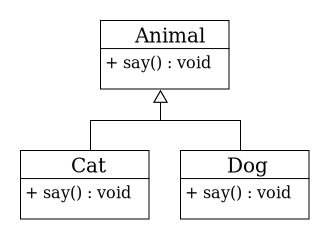
\includegraphics[scale=0.9]{../images/animals.png}
\end{center}
\end{minipage}

\begin{lstlisting}[style=csMiptCppStyle]
int main()
{
    std::vector<Animal*> animals = {new Cat, new Dog, new Dog, new Animal, new Cat};
    
    // В цикле напечатается Meow Woof Woof Hello Meow
    for (auto p : animals)
        p->say();
    
    for (auto p : animals)
        delete p;
}
\end{lstlisting}


\subsection*{Пример использования полиморфизма: Фигуры в 2-х измерениях}
Рассмотрим ещё один похожий пример. Предположим, что мы пишем приложение для работы с 2D графикой и хотим единообразно работать с разными фигурами (кругами, прямоугольниками и т. д.).

\noindent
\begin{minipage}{0.55\textwidth}
\begin{lstlisting}[style=csMiptCppStyle]
#include <iostream>
#include <numbers>
#include <vector>

class Shape
{
public:
    virtual float getArea() const {return 0;}
    virtual ~Shape() {}
};

class Circle : public Shape
{
private:
    float radius;
public:
    Circle(float radius) : radius(radius) {}
    
    float getArea() const override
    {
        return std::numbers::pi * radius * radius;
    }
};
\end{lstlisting}
\end{minipage}
\begin{minipage}{0.45\textwidth}
\begin{center}
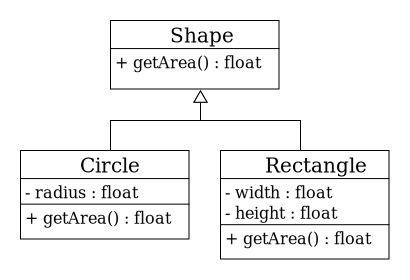
\includegraphics[scale=0.8]{../images/shapes.png}
\end{center}
\end{minipage}

\noindent
\begin{lstlisting}[style=csMiptCppStyle]
class Rectangle : public Shape
{
private:
    float width, height;
public:
    Rectangle(float width, float height) : width(width), height(height) {}
    
    float getArea() const override
    {
        return width * height;
    }
};

int main()
{
    std::vector<Shape*> shapes = {new Rectangle{2, 5}, new Circle(1), new Rectangle{10, 1}};
    
    float areaSum = 0;
    for (auto p : shapes)
        areaSum += p->getArea();
    std::cout << "Sum of areas of all shapes = " << areaSum << std::endl; // 23.1416
    
    for (auto p : shapes)
        delete p;
}
\end{lstlisting}


\subsection*{Хранение указателя на базовый класс в качестве поля другого класса}


\begin{minipage}[t]{0.4\textwidth}
\vspace{10pt}
Ещё одним частым вариантом использования полиморфизма является хранение указателя на базовый класс в полях некоторого другого класса. Такое применение позволяет как бы менять тип поля класса, так как он будет разным в зависимости от того, куда указывает указатель.\\

Дополним предыдущий пример. Предположим, что в нашем приложении можно будет выбирать разные фигуры мышью. Также мы бы хотели, чтобы можно было отменять выбор и возвращаться к предыдущей выбранной фигуре. Для того, чтобы этого добиться, создадим класс \texttt{SelectionState} и будем хранить в нём указатель на текущую выбранную фигуру (\texttt{selectedShape}), а также историю предыдущих выбранных объектов (\texttt{shapeHistory}).\\

Так как \texttt{selectedShape} имеет тип \textit{указатель на базовый класс}  (\texttt{Shape*}), то он может указывать на объекты любых производных классов. Например, этот указатель может указывать на объект типа \texttt{Circle} или на объект типа \texttt{Rectangle}. Мы можем написать код таким образом, чтобы при выборе мышью круга, этот указатель начинал указывать на соответствующий объект типа \texttt{Circle}, а при выборе прямоугольника -- на объект типа \texttt{Rectangle}.\\

Похожим образом мы храним информацию о всех предыдущих выделенных объектах в векторе \texttt{shapeHistory}. Этот вектор состоит из объектов типа \textit{указатель на базовый класс} (\texttt{Shape*}). Некоторые из этих указателей будут указывать на объекты типа \texttt{Circle}, а другие указатели этого вектора будут указывать на объекты типа \texttt{Rectangle} или на объект другого наследника \texttt{Shape}.\\

\vspace{20pt}

\textbf{Использование полиморфизма для реализации паттернов проектирования:}\\
В следующих семинарах мы будем проходить различные паттерны проектирования и динамический полиморфизм это основной мехенизм, используемый при реализации абсолютного большинства паттернов.

\vfill
\end{minipage}
\hfill
\begin{minipage}[t]{0.55\textwidth}
\begin{lstlisting}[style=csMiptCppBorderStyle]
class SelectionState
{
private:
	Shape* selectedShape {nullptr};
	std::vector<Shape*> shapeHistory;
	
public:
	void setSelectedShape(Shape* p)
	{
		shapeHistory.push_back(selectedShape);
		selectedShape = p;
	}
	
	bool undo()
	{
		if (shapeHistory.empty())
			return false;
		delete selectedShape;
		selectedShape = shapeHistory.back();
		shapeHistory.pop_back();
        return true;
	}
	
	float getSelectedArea() const
	{
		if (selectedShape == nullptr)
			return 0;
		return selectedShape->getArea();
	}
	
	~SelectionState()
	{
		delete selectedShape;
		for (auto p : shapeHistory)
			delete p;
	}
};

int main()
{
    SelectionState a;
    a.setSelectedShape(new Circle{10});
    a.setSelectedShape(new Rectangle{5, 2});
    a.setSelectedShape(new Circle{20});
    a.undo();
    std::cout << a.getSelectedArea() << std::endl;
}
\end{lstlisting}
\end{minipage}

\newpage
\subsection*{Полиморфизм и умные указатели}
Одним из больших недостатков предыдущих примеров являлось то, что нам приходилось вручную управлять созданием объектов в куче с помощью \texttt{new} и \texttt{delete}. Это считается не очень хорошей практикой, так как может привести к утечкам памяти или к другим ошибкам работы с памятью. Гораздо более лучший способ -- это использование умных указателей. Умные указатели автоматически уничтожают объект в куче и корректно освобождают память.

Умные указатели стандартной библиотеки \texttt{std::unique\_ptr} и \texttt{std::shared\_ptr} поддерживают полиморфизм. То есть можно указателем типа \textit{умный указатель на базовый класс} указывать на объект производного класса.
Предположим, что у нас есть базовый класс \texttt{Alice} и производный класс \texttt{Bob}. Тогда можно создать умный указатель типа \texttt{std::unique\_ptr<Alice>}, который бы указывал на объект типа \texttt{Bob} следующим образом:
\begin{lstlisting}[style=csMiptCppStyle]
std::unique_ptr<Alice> p = std::make_unique<Bob>();
\end{lstlisting}
Это работает несморя но то, что \texttt{p} имеет тип \texttt{std::unique\_ptr<Alice>}, но инициализируется объектом типа \texttt{std::unique\_ptr<Bob>}.
Дело в том, что в шаблонном классе \texttt{std::unique\_ptr<T>} есть шаблонный конструктор от \texttt{unique\_ptr<OtherT>}, который проверяет, что \texttt{OtherT} является производным классом от нашего типа \texttt{T}.

Перепишем один из прошлых примеров с использованием умного указателя \texttt{std::unique\_ptr}:

\begin{lstlisting}[style=csMiptCppStyle]
#include <iostream>
#include <vector>
#include <memory>

struct Animal
{
    virtual void say() const {std::cout << "Hello" << std::endl;}
    virtual ~Animal() = default;
};

struct Cat : public Animal
{
    void say() const override {std::cout << "Meow" << std::endl;}
};

struct Dog : public Animal
{
    void say() const override {std::cout << "Woof" << std::endl;}
};

int main()
{
    std::vector<std::unique_ptr<Animal>> animals;
    animals.push_back(std::make_unique<Cat>());
    animals.push_back(std::make_unique<Dog>());
    animals.push_back(std::make_unique<Dog>());
    animals.push_back(std::make_unique<Animal>());
    animals.push_back(std::make_unique<Cat>());
    
    // В цикле напечатается Meow Woof Woof Hello Meow
    for (auto& p : animals)
        p->say();
}
\end{lstlisting}
Вектор из \texttt{std::unique\_ptr} к сожалению нельзя инициализировать с помощью фигурных скобочек, так как объекты \texttt{std::unique\_ptr} нельзя копировать, а можно только перемещать. Это особенность/недостаток языка.
Поэтому тут пришлось просто несколько раз использовать \texttt{push\_back}.

\newpage
\section{Реализация механизма виртуальных функций}
\subsection*{Как программа понимает, какой виртуальный метод вызывать}
Размер объектов полиморфных типов. Скрытый указатель на таблицу виртуальных функций.


\subsection*{Схема механизма виртуальных функций}
\noindent\begin{minipage}{.43\textwidth}
\begin{lstlisting}[style=csMiptCppStyle]
#include <iostream>
struct Alice 
{
	int x;
    virtual void say() 
    {
    	std::cout << "Alice Say\n";
    }
    virtual void walk() 
    {
    	std::cout << "Alice Walk\n";
    }
};

struct Bob : public Alice 
{
	int y;
    void say() override
    {
    	std::cout << "Bob Say\n";
    }
    void walk() override
    {
    	std::cout << "Bob Walk\n";
    }
};

int main() 
{
    Alice a {10};
    Bob b {20, 30};
    
    Alice* p = &a;
    p->say();  // Напечатает Alice Say
    
    p = &b;
    p->say();  // Напечатает Bob Say
}
\end{lstlisting}
\end{minipage}
\begin{minipage}{.5\textwidth}
\includegraphics[scale=0.75]{../images/virtual_table_alice_bob.png}
\end{minipage}

\newpage
\section{Абстрактные классы и интерфейсы}
\subsection*{Чистые виртуальные функции}
\textbf{Чистая виртуальная функция} (англ. \textit{pure virtual function}) -- это виртуальная функция, в объявлении которой прописывается, то что она "равна нулю"{}, например вот так:
\begin{lstlisting}
virtual void say() = 0;
\end{lstlisting}
У таких функций, как правило, нет определения и они не предназначены для того, чтобы их вызывали. Единственная их цель заключается в том, чтобы эти функции были переопределены в классах наследниках.
\subsection*{Абстрактные классы}
\textbf{Абстрактный класс} -- это класс у которого есть хотя бы одна чистая виртуальная функция (либо своя, либо отнаследованная). Объект абстрактного класса нельзя создать. Такие классы предзазначены только для того, чтобы от них наследоваться.
\begin{lstlisting}
#include <iostream>
struct Alice 
{
    virtual void say() = 0;
    virtual ~Alice() {}
};

struct Bob : public Alice 
{
    void say() override
    {
    	std::cout << "Bob" << std::endl;
    }
};

int main()
{
	Alice a;              // Ошибка: нельзя создать объект класса Alice
	Alice* p = new Alice; // Ошибка: нельзя создать объект класса Alice
	
	Alice* q = new Bob;   // ОК
	q->say();             // Напечатает Bob
	delete q;
}
\end{lstlisting}

\subsection*{Интерфейс}
\textbf{Интерфейс} -- это абстрактный класс, у которого нет полей, в все методы (за исключением, быть может, деструктора) -- чистые виртуальные методы.

\subsection*{pure virtual call и определение чистых виртуальных методов}


\newpage
\section{RTTI и \texttt{dynamic\_cast}}
\subsection*{Полиморфный тип}
\subsection*{\texttt{dynamic\_cast}}

\subsubsection*{\texttt{dynamic\_cast} от родителя к ребёнку}
\subsubsection*{\texttt{dynamic\_cast} в бок}

\subsection*{Оператор \texttt{typeid} и класс \texttt{std::type\_info}}


\end{document}
